\subsection{连续函数}

定义 1. 映射 \(f\)（由拓扑空间 \(\mathbf{X}\) 到拓扑空间 \(\mathbf{X}'\) 中的映射）称为在点 \(x_0 \in \mathbf{X}\) 处连续，如果对任一邻域 \(\mathbf{V}'\)（\(f(x_0)\) 在 \(\mathbf{X}'\) 中的邻域），存在一个邻域 \(\mathbf{V}\)（\(x_0\) 在 \(\mathbf{X}\) 中的邻域），使得关系 \(x \in \mathbf{V}\) 蕴含 \(f(x) \in \mathbf{V}'\)。

定义 1 可以改述为下列更直观的形式：说 \(f\) 在点 \(x_0\) 处连续，意思是 \(f(x)\) 可以随意地接近 \(f(x_0)\)，只要 \(x\) 充分接近 \(x_0\)。

关系“对每个 \(x \in V\)，\(f(x) \in V'\)”等价于 \(f(V) \subset V'\)，或者再等价于 \(V \subset \overline{f}^{1}(V')\)；鉴于邻域公理 \((V_{I})\)，我们看到定义 1 等价于下述定义：称 \(f: X \to X'\) 在点 \(x_{0}\) 处连续，如果对每个邻域 \(V'\)（\(f(x_{0})\) 在 \(X'\) 中的邻域），\(\overline{f}^{1}(V')\) 是 \(x_{0}\) 在 X 中的邻域。而且，只需 \(\overline{f}^{1}(V')\) 是 \(x_{0}\) 的邻域（对每个邻域 \(V'\)，它属于 \(f(x_{0})\) 在 \(X'\) 中的某个基本邻域系）就够了（§ 1，第 3 目）。

命题 1. 设 \(f\) 是由拓扑空间 \(\mathbf{X}\) 到拓扑空间 \(\mathbf{X}'\) 中的一个映射。如果 \(f\) 在 \(x\) 处连续，并且 \(x\) 位于子集 \(A\)（\(X\) 的子集）的闭包中，则 \(f(x)\) 位于 \(f(A)\) 的闭包中。

设 \(\mathbf{V}'\) 是 \(f(x)\) 在 \(\mathbf{X}'\) 中的一个邻域。由于 \(f\) 在 \(x\) 处连续，\(\overline{f}^1 (\mathbf{V}')\) 是 \(x\) 在 \(\mathbf{X}\) 中的邻域。于是 \(\overline{f}^1 (\mathbf{V}')\) 与 \(\mathbf{A}\) 相交，由此推出 \(\mathbf{V}'\) 与 \(f(\mathbf{A})\) 相交，从而 \(f(x)\) 位于 \(f(\mathbf{A})\) 的闭包中。

命题 2. 设 X、X'、X'' 是三个拓扑空间；设 f 是由 X 到 X' 中的映射，在 x ∈ X 处连续；设 g 是由 X' 到 X'' 中的映射，在 f(x) 处连续。则复合映射 h = g \(\circ\) f: X → X'' 在 x 处连续。

设 \(V''\) 是 \(h(x) = g(f(x))\) 在 \(X''\) 中的一个邻域。由于 \(g\) 在 \(f(x)\) 处连续，可知 \(\overline{g}^1(V'')\) 是 \(f(x)\) 在 \(X'\) 中的邻域。但 \(f\) 在 \(x\) 处连续，故 \(\overline{f}^1(\overline{g}^1(V'')) = \overline{h}^1(V'')\) 是 \(x\) 在 \(X\) 中的邻域，从而 \(h\) 在 \(x\) 处连续。

定义 2. 由拓扑空间 X 到拓扑空间 X' 中的映射称为在 X 上连续（或简称连续），如果它在 X 的每一点都连续。

例。1) 拓扑空间 X 到自身的恒等映射是连续的。

\begin{enumerate}
\def\labelenumi{\arabic{enumi})}
\setcounter{enumi}{1}
\item
  拓扑空间到拓扑空间中的常映射是连续的。
\item
  由离散空间到拓扑空间中的每个映射都是连续的。
\end{enumerate}

定理 1. 设 \(f\) 是由拓扑空间 \(X\) 到拓扑空间 \(X'\) 中的一个映射。则下列命题等价：

\begin{enumerate}
\def\labelenumi{\alph{enumi})}
\item
  \(f\) 在 \(\mathbf{X}\) 中连续。
\item
  对 X 的每个子集 A，\(f(\overline{\mathrm{A}}) \subset \overline{f(\mathrm{A})}\)。
\item
  在 \(f\) 之下，\(\mathbf{X}'\) 的每个闭子集的逆像是 \(\mathbf{X}\) 的闭子集。
\item
  在 \(f\) 之下，\(\mathbf{X}'\) 的每个开子集的逆像是 \(\mathbf{X}\) 的开子集。
\end{enumerate}

我们已经看到 a) 蕴含 b)（命题 1）。为证 b) 蕴含 c)，设 \(\mathbf{F}'\) 是 \(\mathbf{X}'\) 的闭子集，并设 \(\mathbf{F} = \overline{f}^{1}(\mathbf{F}')\)；则由假设 \(f(\overline{\mathbf{F}}) \subset \overline{f(\mathbf{F})} \subset \overline{\mathbf{F}}' = \mathbf{F}'\)，故 \(\overline{\mathbf{F}} \subset \overline{f}^{1}(\mathbf{F}') = \mathbf{F} \subset \overline{\mathbf{F}}\)，于是 \(\mathbf{F} = \overline{\mathbf{F}}\)，即 \(\mathbf{F}\) 是闭集。鉴于关系式 \(\complement \overline{f}^{1}(A') = \overline{f}^{1}(\complement A')\)（对每个子集 \(A'\)（\(X'\) 的子集）成立），c) 蕴含 d)。最后，设 d) 成立。设 \(x\) 是 \(X\) 的任一点，并设 \(V'\) 是 \(f(x)\) 在 \(X'\) 中的任一邻域；则存在开集 \(A'\)（\(X'\) 中的），使得

\[
f (x) \in \mathrm{A} ^ {\prime} \subset \mathrm{V} ^ {\prime}
\]

从而 \(x \in \overline{f}^1(\mathbf{A}') \subset \overline{f}^1(\mathbf{V}')\)。由假设，\(\overline{f}^1(\mathbf{A}')\) 在 \(\mathbf{X}\) 中是开集，于是 \(\overline{f}^1(\mathbf{V}')\) 是 \(x\) 在 \(\mathbf{X}\) 中的邻域。这样 d) 蕴含 a)。

注。1) 设 \(\mathfrak{B}\) 是 \(\mathbf{X}'\) 的拓扑的一个拓扑基（§ 1，第 3 目）；则为使 \(f: \mathbf{X} \to \mathbf{X}'\) 连续，必要且充分的是：\(\overline{f}^1(\mathbf{U}')\) 在 \(\mathbf{X}\) 中是开集（对每个 \(\mathbf{U}' \in \mathfrak{B}\)）。

例。设 \(a\) 是任一有理数。映射 \(x \to a + x\)（由有理直线 \(\mathbf{Q}\) 到自身的映射）在 \(\mathbf{Q}\) 上连续，因为开区间 \(]b, c[\) 在该映射下的逆像是开区间

\[
] b - a, c - a [.
\]

同样，映射 \(x \to ax\) 在 \(\mathbf{Q}\) 上连续；若 \(a = 0\) 这是显然的，因为此时 \(ax = 0\) 对所有 \(x\) 成立；若 \(a \neq 0\)，则开区间 \(]b, c[\) 在该映射下的逆像是以 \(b / a\) 与 \(c / a\) 为端点的开区间。

\pandocbounded{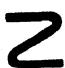
\includegraphics[keepaspectratio]{images/part001_4077020d.jpg}}

\begin{enumerate}
\def\labelenumi{\arabic{enumi})}
\setcounter{enumi}{1}
\tightlist
\item
  在连续映射 \(f: \mathbf{X} \to \mathbf{X}'\) 下，X 的开（相应地，闭）集的直接像在 \(\mathbf{X}'\) 中未必是开（相应地，闭）集（参见 § 5）。
\end{enumerate}

例。* 映射 \(f: x \to 1 / (1 + x^2)\)（由 \(\mathbf{R}\) 到自身的映射）是连续的，但 \(f(\mathbf{R})\) 是半开区间 {[}0, 1{]}，它在 \(\mathbf{R}\) 中既不是开集也不是闭集。*

定理 2. 1) 如果 \(f: \mathbf{X} \to \mathbf{X}'\) 与 \(g: \mathbf{X}' \to \mathbf{X}''\) 是两个连续映射，则 \(g \circ f: \mathbf{X} \to \mathbf{X}''\) 连续。

\begin{enumerate}
\def\labelenumi{\arabic{enumi})}
\setcounter{enumi}{1}
\tightlist
\item
  为使双射 \(f\)（由拓扑空间 \(X\) 到拓扑空间 \(X'\) 上的双射）是同胚，必要且充分的是 \(f\) 与 \(f\) 的逆都连续（或者说，\(f\) 是双连续的）。
\end{enumerate}

第一个断言是命题 2 的直接推论；第二个断言由定理 1 的 d) 与同胚的定义（§ 1，第 1 目）得出。

\pandocbounded{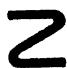
\includegraphics[keepaspectratio]{images/part001_720050f1.jpg}}

注。1) 可能存在由拓扑空间 X 到拓扑空间 X' 上的连续双射而不是双连续的：例如，取 X' 为有理直线 Q，取 X 为赋予离散拓扑的集合 Q；则恒等映射 X → X' 连续但不是同胚。

\begin{enumerate}
\def\labelenumi{\arabic{enumi})}
\setcounter{enumi}{1}
\item
  为验证连续双射 \(f: \mathbf{X} \to \mathbf{X}'\) 是同胚，只需证明：对每个 \(x \in \mathbf{X}\) 与每个邻域 \(V\)（\(x\) 的邻域），\(f(V)\) 是 \(f(x)\) 在 \(\mathbf{X}'\) 中的邻域。
\item
  设 X 是拓扑空间，对每个 \(x \in X\)，设 \(\mathfrak{B}(x)\) 是 x 的所有邻域所成之集。设 \(x_{0}\) 是 X 的一点；对每个 \(x \in X\)，按如下方式定义 X 的子集所成之集 \(\mathfrak{B}_{0}(x)\)：\(\mathfrak{B}_{0}(x_{0}) = \mathfrak{B}(x_{0})\)，而若 \(x \neq x_{0}\)，则 \(\mathfrak{B}_{0}(x)\) 取为 X 的包含 x 的所有子集所成之集。立即可以验证（§ 1，第 2 目，命题 2），诸集 \(\mathfrak{B}_{0}(x)\) 是 X 上某个拓扑的诸点的邻域集；用 \(X_{0}\) 表示这样得到的拓扑空间，用 \(j : X_{0} \to X\) 表示恒等映射，它连续但一般不是双连续的。X 到拓扑空间 \(X'\) 中的映射 f 在点 \(x_{0}\) 处连续当且仅当复合映射 \(X_{0} \stackrel{j}{\to} X \stackrel{f}{\to} X'\) 在 \(X_{0}\) 上连续；这由定义立即得出。
\end{enumerate}

